\label{method_positioning}

\subsection{Ước tính quãng đường di chuyển dựa trên bộ đếm bước và khoảng cách liên chi}

\subsubsection{Bộ lọc tầng 1—Giới hạn phạm vi khoảng cách và góc quét}

\begin{figure}[b!]
    \centering
    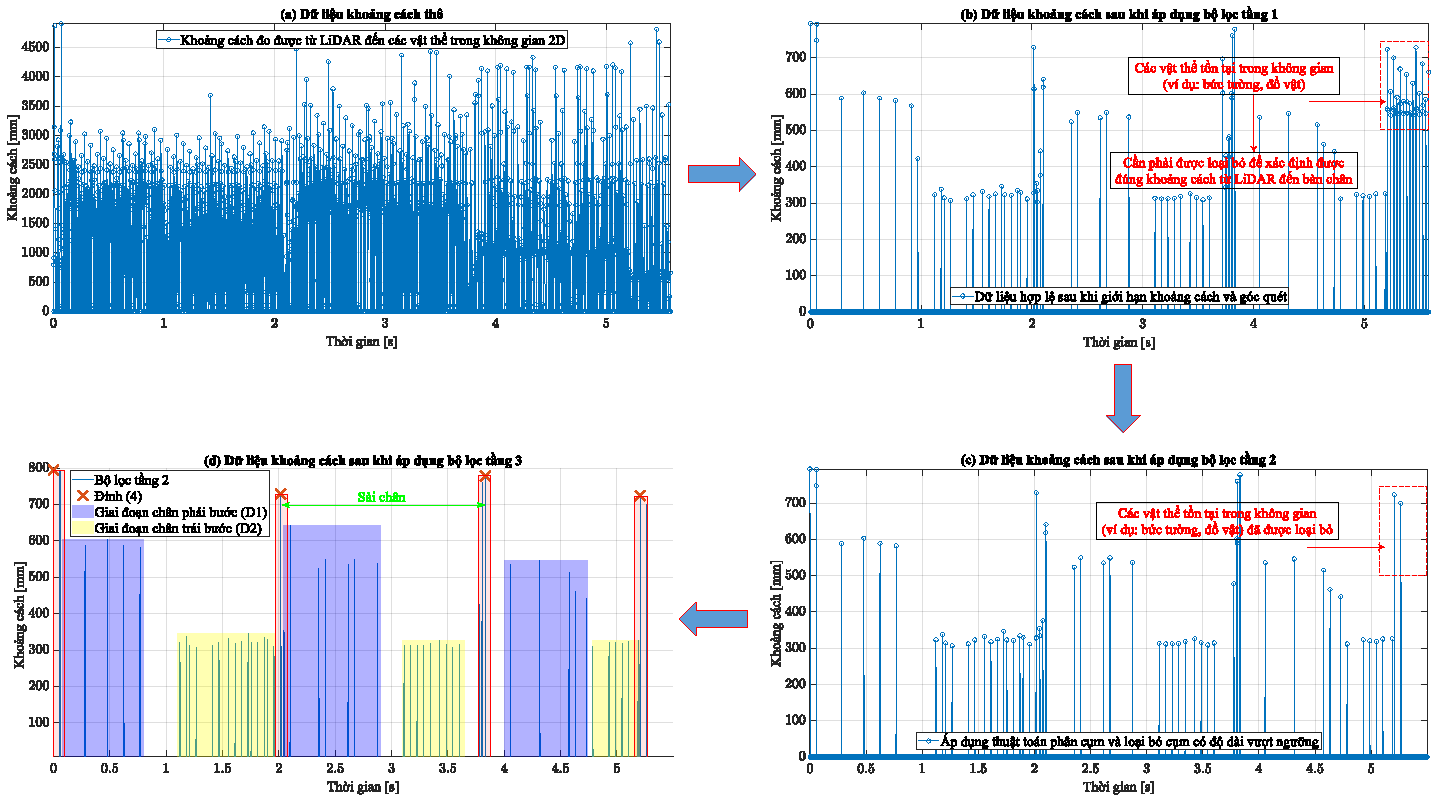
\includegraphics[width=1\linewidth]{Figure/lidar_bo_loc.pdf}
    \caption{Một bộ lọc đa giai đoạn nhằm trích xuất khoảng cách liên chi dựa trên LiDAR}
    \label{lidar_bo_loc}
\end{figure}

Hệ thống định vị sử dụng cảm biến LiDAR, gắn tại chân phải của nhân viên cứu hộ, nhằm mục đích đo khoảng cách giữa cảm biến và chân trái. Mặc dù LiDAR có khả năng cung cấp dữ liệu với độ chính xác cao, trong quá trình di chuyển, dữ liệu thu thập được vẫn chứa nhiều điểm nhiễu và không thể xác định rõ ràng đâu là điểm đại diện cho bước chân. Điều này tạo ra sự khó khăn trong việc xác định chính xác độ dài bước chân từ cảm biến. Dữ liệu thô thu được từ cảm biến LiDAR sẽ chứa nhiều giá trị không cần thiết do ảnh hưởng của các yếu tố môi trường hoặc chuyển động của cơ thể. Nhằm cải thiện khả năng xác định khoảng cách đến chân trái, quá trình lọc bước đầu tiên được thực hiện để loại bỏ các điểm dữ liệu không hợp lệ.

Hình~\ref{lidar_bo_loc}a mô tả dữ liệu khoảng cách thu được từ cảm biến theo thời gian trong một khoảng 5,5 giây, trong đó có 6 bước chân được thực hiện. Dữ liệu này có khoảng cách đo được lên đến 5.000~mm, nhưng chưa qua xử lý, việc phân biệt đâu là khoảng cách thực sự từ cảm biến đến chân trái là rất khó khăn. Do đó, cần thiết phải áp dụng bộ lọc đầu tiên để làm sạch dữ liệu và giúp việc xác định khoảng cách trở nên rõ ràng hơn. Trong quá trình lọc tầng 1, hệ thống sử dụng các điều kiện sau (Hình~\ref{lidar_bo_loc_tang_1_2}a):

\begin{boxlabel}
    \item Giới hạn góc quét: Cảm biến LiDAR chỉ quét trong phạm vi từ 0$^\circ$ đến 180$^\circ$, vì đây là phạm vi có thể đo được khoảng cách đến chân trái khi di chuyển. Các giá trị khoảng cách ngoài phạm vi này sẽ được gán bằng 0, vì không có khả năng đo được chân trái.
    
    \item Giới hạn khoảng cách: Cảm biến có thể trả về giá trị khoảng cách lên đến 12~m, tuy nhiên, khoảng cách này sẽ được giới hạn trong phạm vi từ 200~mm đến 800~mm. Các giá trị nằm ngoài phạm vi này cũng sẽ bị gán bằng 0, vì chúng không phản ánh được sự thay đổi về khoảng cách giữa cảm biến và chân trái trong quá trình di chuyển.
\end{boxlabel}

\begin{figure}[t]
    \centering
    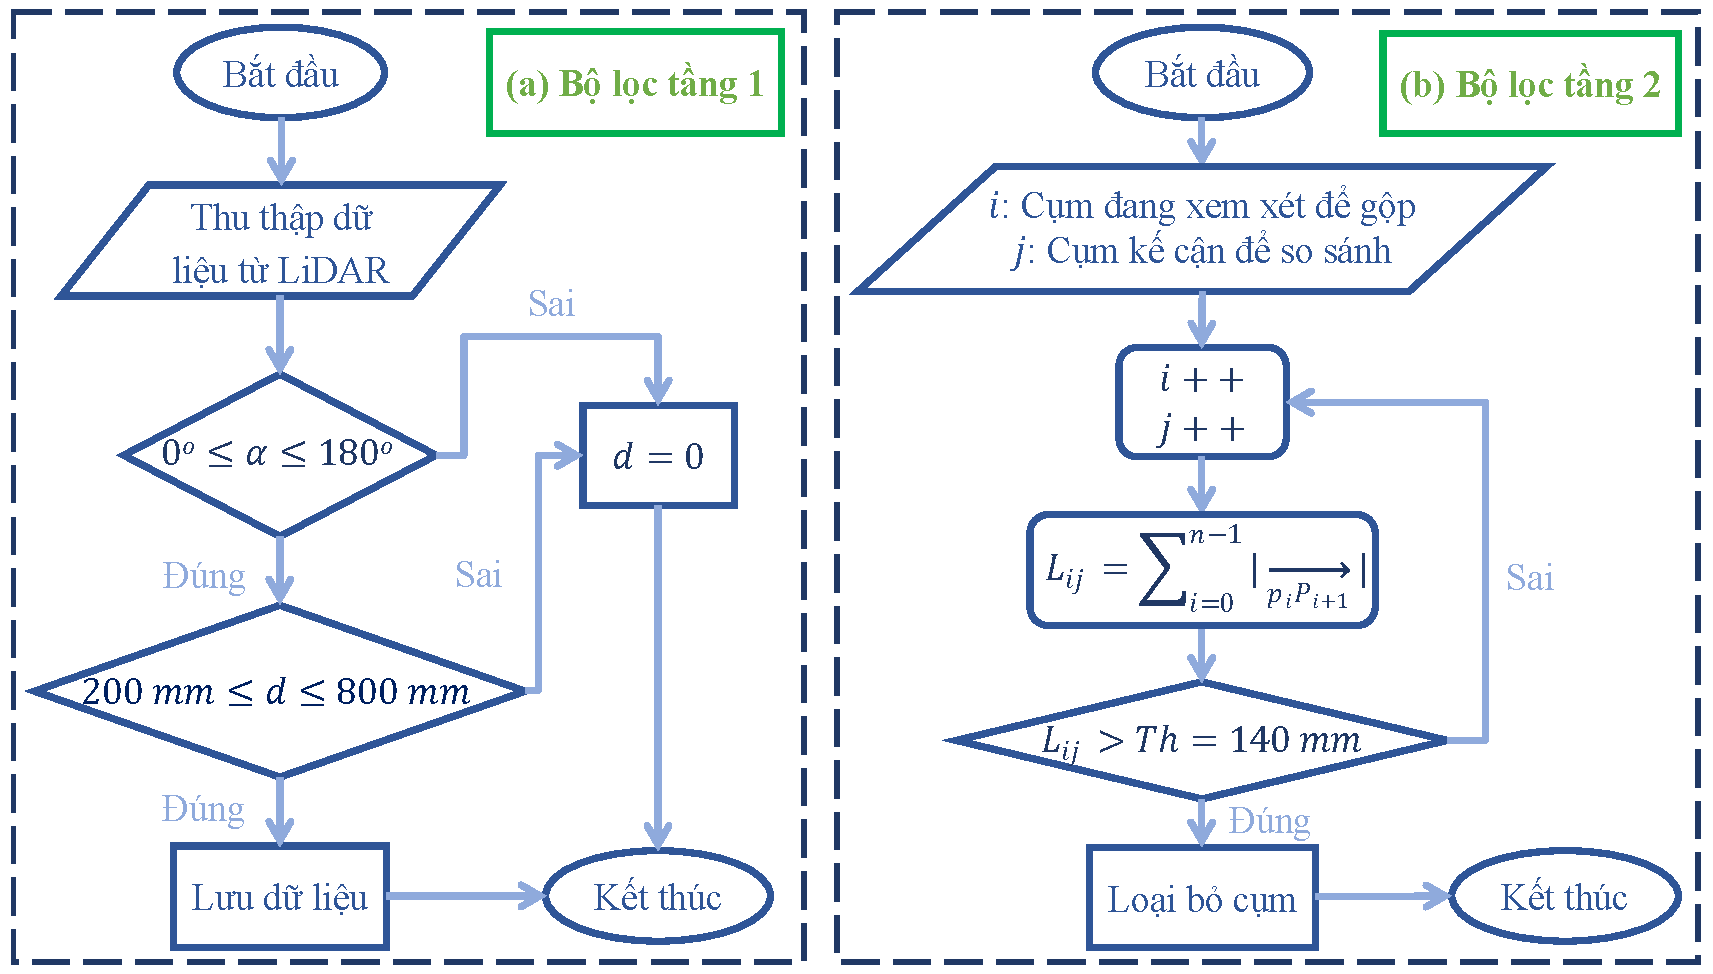
\includegraphics[width=1\linewidth]{Figure/lidar_bo_loc_tang_1_2.pdf}
    \caption{Lưu đồ thuật toán (a) Bộ lọc tầng 1 và (b) Bộ lọc tầng 2}
    \label{lidar_bo_loc_tang_1_2}
\end{figure}

Sau khi áp dụng bộ lọc tầng 1, dữ liệu đã được làm sạch và giảm thiểu nhiễu, như thể hiện trong hình~\ref{lidar_bo_loc}b. Dữ liệu sau khi lọc bớt độ dày và dễ dàng quan sát hơn, từ đó tạo nền tảng vững chắc cho các bước tiếp theo trong việc xác định độ dài bước chân và quãng đường di chuyển.

\subsubsection{Bộ lọc tầng 2—Phân cụm dữ liệu và loại bỏ các đỉnh dương tính giả}

Dữ liệu thu được từ cảm biến LiDAR có tính chất tuần hoàn, với các giá trị đo được lặp lại theo chu kỳ từ 0$^\circ$ đến 360$^\circ$. Điều này dẫn đến việc các điểm dữ liệu có khả năng xuất hiện nhiều lần tại các góc khác nhau nhưng vẫn có cùng giá trị khoảng cách, gây khó khăn trong việc phân tách dữ liệu bước chân và các điểm nhiễu (như bức tường, đồ vật). Để khắc phục vấn đề này, hệ thống áp dụng bộ lọc tầng 2, sử dụng thuật toán phân cụm nhằm tách biệt dữ liệu bước chân với các điểm nhiễu không mong muốn (Hình~\ref{lidar_bo_loc_tang_1_2}b).

\paragraph{Phân đoạn dữ liệu}

Trước tiên, dữ liệu thu được từ cảm biến được phân đoạn thành các cửa sổ trượt với kích thước 100 mẫu và độ chồng lấp 50 \%. Việc áp dụng phân đoạn dữ liệu nhằm đảm bảo mỗi đoạn chỉ chứa các điểm trong một khoảng thời gian ngắn, từ đó giúp tách biệt dữ liệu bước chân khỏi các vật thể cố định và giảm thiểu khả năng nhiễu. Nếu không thực hiện phân đoạn, dữ liệu sẽ được xử lý liên tục theo thời gian, dẫn đến nguy cơ các điểm nhiễu có khả năng bị gom nhầm vào cụm dữ liệu bước chân, làm giảm độ chính xác của quá trình phân cụm (Hình~\ref{cluster_data}a). Sau khi áp dụng phương pháp phân đoạn bằng cửa sổ trượt, các điểm nhiễu, chẳng hạn như bức tường hoặc các cấu trúc môi trường cố định, có xu hướng nằm trên các đường thẳng, đặc trưng cho các vật thể không di chuyển và phản ánh đặc điểm không thay đổi theo thời gian của các vật thể này (Hình~\ref{cluster_data}b).

\paragraph{Ánh xạ dữ liệu từ hệ tọa độ cực sang hệ tọa độ Descartes}

\begin{figure}[b!]
    \centering
    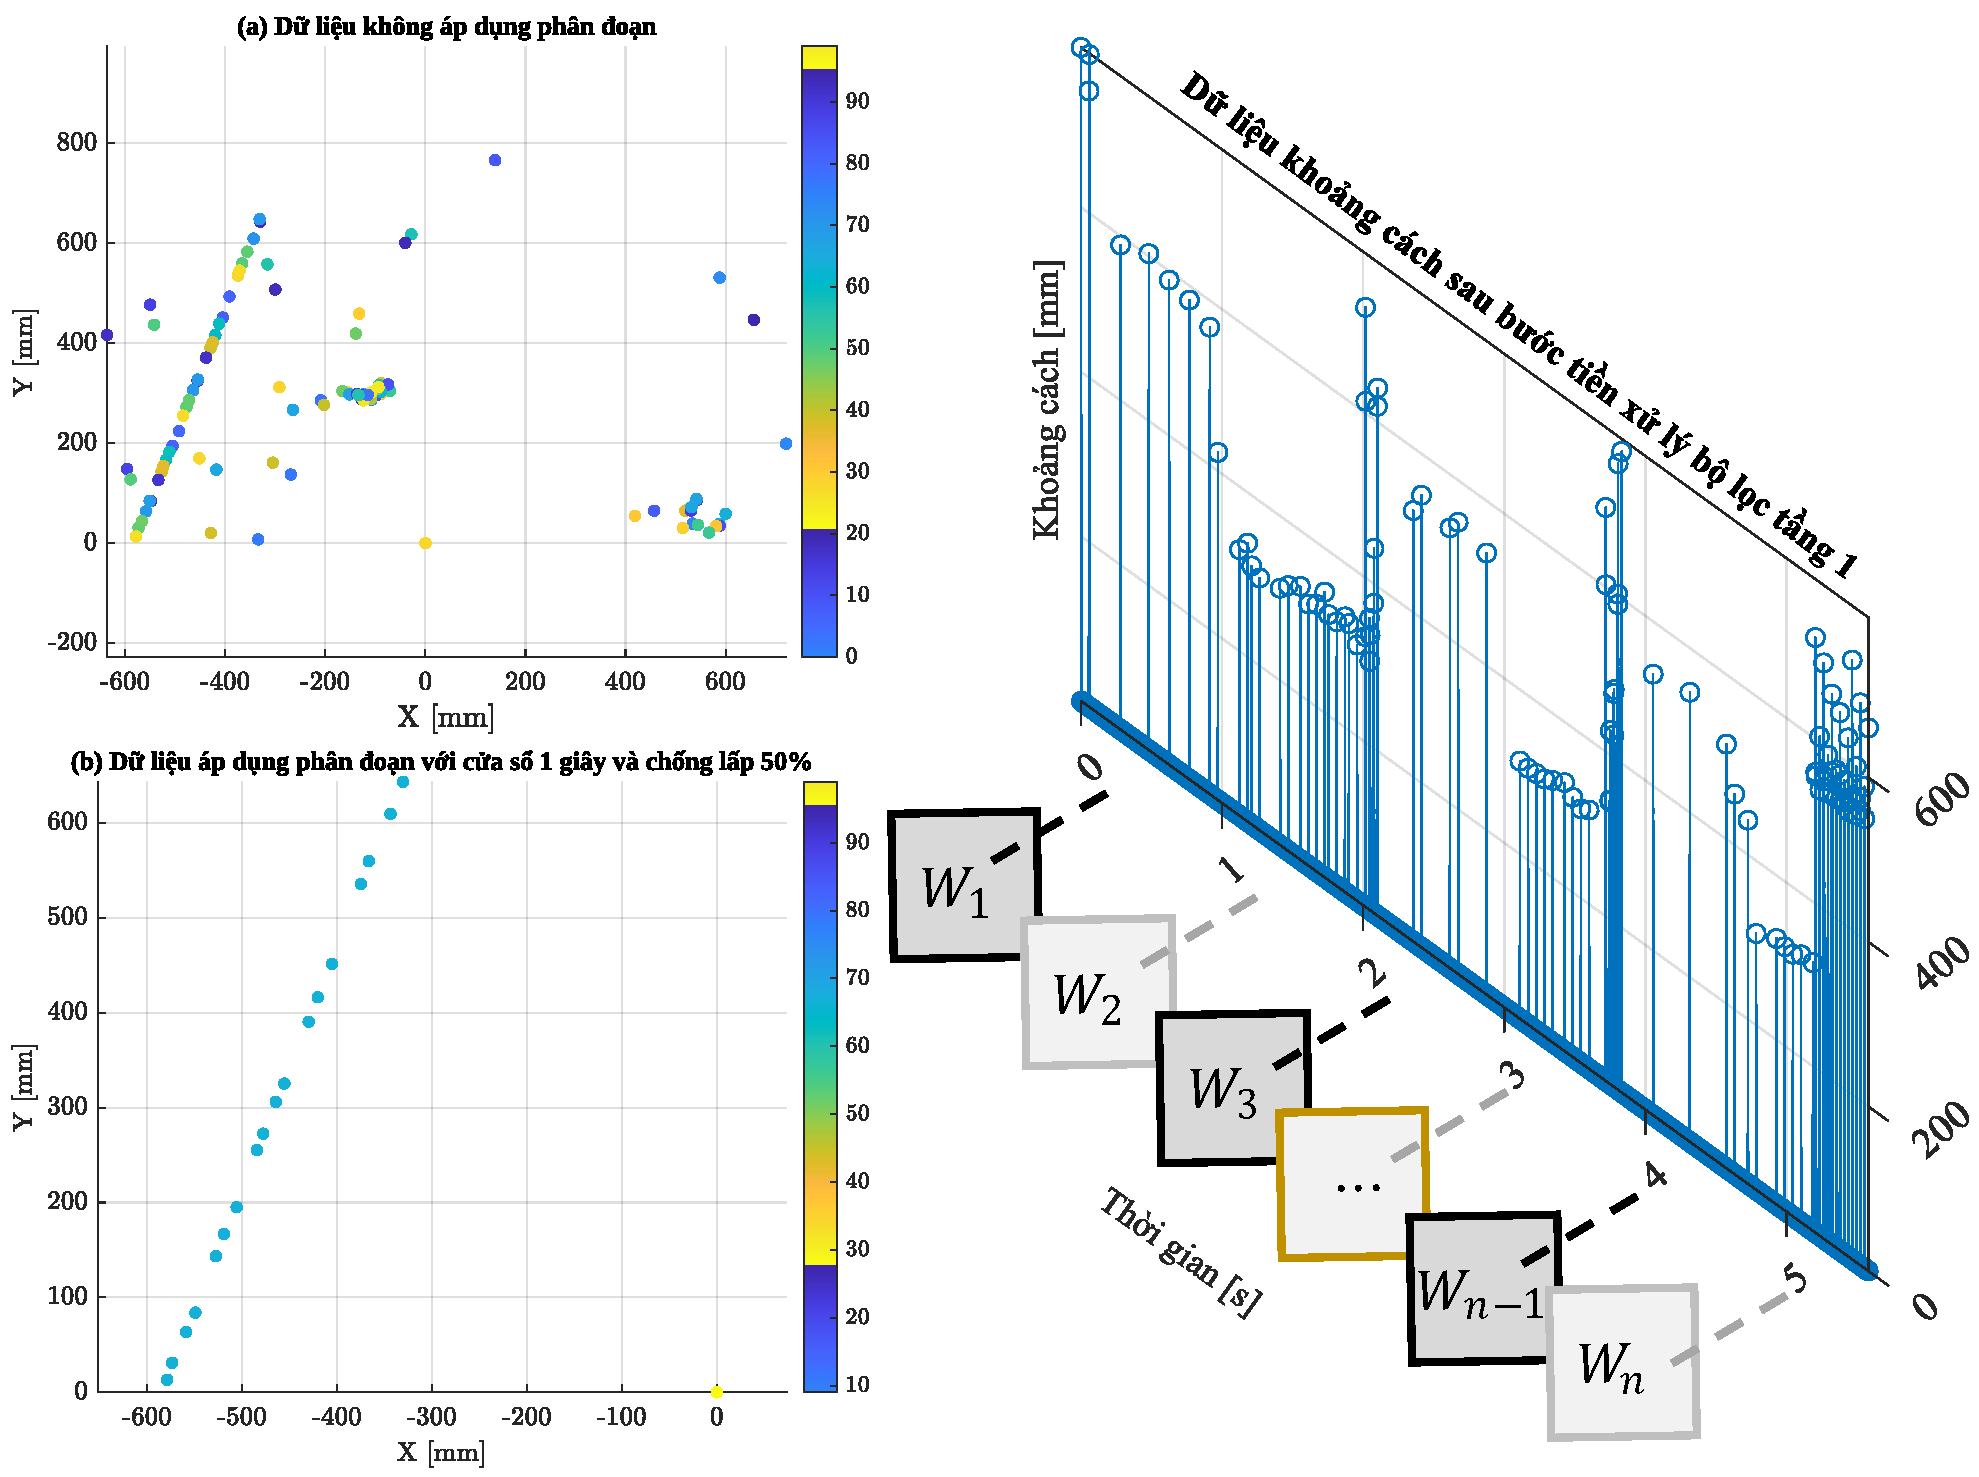
\includegraphics[width=1\linewidth]{Figure/cluster_data.pdf}
    \caption{Dữ liệu khoảng cách và góc (hệ tọa độ cực) được ánh xạ sang hệ tọa độ Descartes: (a) Dữ liệu không áp dụng phân đoạn; (b) Dữ liệu áp dụng phân đoạn cửa sổ 1 giây và chồng lấp 50 \%}
    \label{cluster_data}
\end{figure}

Trong mỗi cửa sổ dữ liệu, các điểm dữ liệu $P_n = (D_n, \alpha_n)$, trong đó $D_n$ là khoảng cách và $\alpha_n$ là góc đo được từ cảm biến, được chuyển đổi sang tọa độ Descartes $P_n = (x_n, y_n)$ như sau \eqref{mapped_descartes}:

\begin{equation}
    x_n = D_n \cdot \cos(\alpha_n), \quad y_n = D_n \cdot \sin(\alpha_n)\label{mapped_descartes}
\end{equation}
Hình~\ref{cluster_data}b mô tả một cửa sổ dữ liệu thứ 54 sau khi phân đoạn và ánh xạ sang hệ tọa độ $\mathrm{Oxy}$.

\paragraph{Phân cụm dữ liệu}

Sau khi ánh xạ, các điểm dữ liệu trong từng cửa sổ được phân cụm dựa trên khoảng cách Euclidean $K$ giữa các điểm. Một thuật toán phân cụm dựa trên tìm kiếm theo chiều rộng (Breadth-First Search - BFS) được sử dụng để nhóm các điểm gần nhau dựa trên hai ngưỡng: độ lệch góc dưới 10° và khoảng cách Euclidean với hai điểm $p_i$ và $p_j$ trong cùng một cụm phải thỏa mãn điều kiện sau \eqref{k_euclidean}:

\begin{equation}
    K = \sqrt{(x_i - x_j)^2 + (y_i - y_j)^2} \leq D_{\text{min}}\label{k_euclidean}
\end{equation}
trong đó $D_{\text{min}} =$ 100~mm là ngưỡng khoảng cách tối thiểu để các điểm được nhóm vào cùng một cụm. Nếu $D_{\text{min}}$ được thiết lập quá lớn, các điểm dữ liệu nhiễu (như các điểm trên bức tường hoặc vật thể cố định) có thể bị gom nhầm vào cụm bước chân, dẫn đến việc dữ liệu bước chân bị che khuất. Ngược lại, nếu $D_{\text{min}}$ quá nhỏ, các cụm dữ liệu bước chân sẽ bị phân chia thành nhiều cụm nhỏ, làm giảm tính liên tục của dữ liệu bước chân.

% Sau khi các cụm dữ liệu ban đầu được hình thành dựa trên khoảng cách Euclidean giữa các điểm dữ liệu, thuật toán tiếp tục thực hiện quá trình gộp cụm nhằm giảm thiểu sự phân mảnh của các cụm nhỏ và rời rạc. Trong bước này, mỗi cụm dữ liệu được đại diện bởi một điểm duy nhất, gọi là \textit{“centroid”}. Centroid của từng cụm được xác định bằng cách tính toán giá trị trung bình của tất cả các điểm dữ liệu trong cụm đó theo \eqref{centroid}:

% \begin{equation}
%     \text{centroid}_k = \left(\frac{\sum_{i=1}^{n_k} x_i}{n_k}, \frac{\sum_{i=1}^{n_k} y_i}{n_k} \right)\label{centroid}
% \end{equation}
% trong đó $n_k$ là số điểm dữ liệu trong cụm $k$ và $(x_i, y_i)$ là tọa độ Descartes của từng điểm dữ liệu trong cụm. Việc tính toán centroid không chỉ giúp đại diện hóa cụm dữ liệu bằng một điểm duy nhất mà còn giảm thiểu độ phức tạp trong quá trình so sánh khoảng cách giữa các cụm. Thay vì tính toán khoảng cách giữa từng cặp điểm dữ liệu trong hai cụm, phương pháp này chỉ cần so sánh khoảng cách giữa hai centroid. Điều này giúp tiết kiệm tài nguyên tính toán, đặc biệt khi số lượng điểm dữ liệu trong mỗi cụm lớn.

% Sau khi xác định centroid cho từng cụm, thuật toán tiến hành so sánh khoảng cách giữa từng cặp centroid $(i, j)$ để đánh giá khả năng gộp cụm. Hai cụm sẽ được xem xét để gộp lại nếu khoảng cách giữa hai centroid nhỏ hơn một ngưỡng $\delta_{\text{merge}}$, được thiết lập ở mức 50~mm. Ngưỡng này được xác định thông qua khảo sát thực nghiệm, đảm bảo chỉ các cụm dữ liệu gần nhau mới được gộp lại. Nếu khoảng cách giữa hai centroid nhỏ hơn 50~mm, hai cụm dữ liệu sẽ được kết hợp thành một cụm duy nhất, từ đó giảm thiểu sự xuất hiện của các cụm nhỏ, rời rạc. Ngược lại, nếu khoảng cách lớn hơn ngưỡng, các cụm dữ liệu sẽ được duy trì như các cụm độc lập.

% Phương pháp gộp cụm không chỉ giúp duy trì tính liên tục của các cụm dữ liệu bước chân mà còn loại bỏ các cụm nhiễu có kích thước nhỏ hoặc có sự phân bố không đồng nhất. Điều này đặc biệt quan trọng trong bối cảnh môi trường có sự xuất hiện của các vật thể cố định, vốn có khả năng tạo ra các cụm dữ liệu không liên quan đến bước chân. Kết quả của quá trình gộp cụm là một tập hợp các cụm dữ liệu đã được tối ưu hóa về mặt cấu trúc và tính liên tục, từ đó giảm thiểu tác động của các cụm nhiễu và tăng cường khả năng phát hiện và nhận diện dữ liệu bước chân.

\paragraph{Tính chiều dài cụm}

Sau khi phân cụm, chiều dài của mỗi cụm được tính toán bằng tổng khoảng cách Euclidean giữa các điểm liên tiếp trong cụm \eqref{euclidean_distance}:

\begin{equation}
    \mathcal{L} = \sum_{i=0}^{n-1} \left| \overrightarrow{p_i p_{i+1}} \right|\label{euclidean_distance}
\end{equation}
trong đó $\mathcal{L}$ là chiều dài của cụm, $p_i$ là các điểm đã được ánh xạ sang hệ tọa độ $\mathrm{Oxy}$ và $n$ là số điểm trong cụm. Giá trị $\left| \overrightarrow{p_i p_{i+1}} \right|$ biểu thị khoảng cách Euclidean giữa hai điểm liên tiếp $p_i$ và $p_{i+1}$ trong không gian 2D.

Các cụm có chiều dài $\mathcal{L}$ vượt quá ngưỡng $\theta =$ 140~mm sẽ bị loại bỏ. Ngưỡng này được thiết lập dựa trên khảo sát thực nghiệm nhằm loại bỏ các cụm dữ liệu có khả năng là bức tường hoặc các vật thể cố định, vì chúng thường có chiều dài lớn hơn dữ liệu bước chân. Sau khi áp dụng quy trình lọc, dữ liệu bước chân sẽ được làm sạch và loại bỏ các cụm nhiễu, chỉ giữ lại các cụm có chiều dài nhỏ hơn $\theta$, từ đó giảm thiểu tác động của các vật thể không mong muốn và tăng cường khả năng nhận diện chuyển động bước chân. Kết quả là hình~\ref{lidar_bo_loc}c thể hiện dữ liệu bước chân đã được làm sạch sau khi áp dụng bộ lọc tầng 2 bằng phương pháp phân cụm.

\subsubsection{Bộ lọc tầng 3—Tăng cường nhận diện các đỉnh nổi bật}

Để xác định khoảng cách từ cảm biến LiDAR đến chân trái, phương pháp phát hiện đỉnh được áp dụng (Hình~\ref{lidar_bo_loc_tang_3_trigonometric}a). Khi chân phải (chân gắn cảm biến) bước lên, các điểm quét được ở chân trái sẽ tạo thành các dao động bất thường trong dữ liệu quét. Điều này cho phép nhận diện các đỉnh—các điểm mà giá trị đo khoảng cách đạt cực đại so với các điểm lân cận.

\begin{figure}[t]
    \centering
    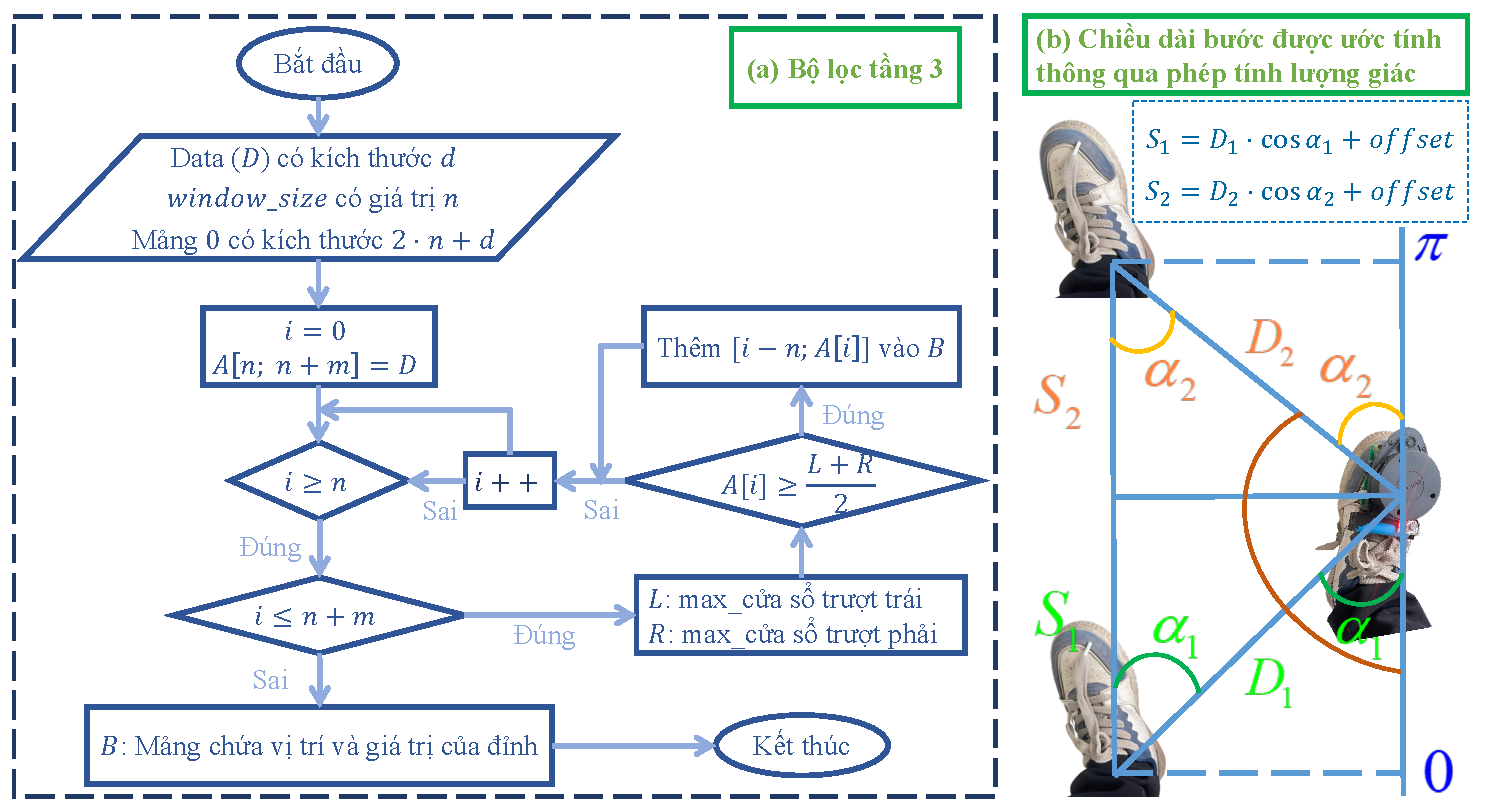
\includegraphics[width=1\linewidth]{Figure/lidar_bo_loc_tang_3_trigonometric.pdf}
    \caption{(a) Lưu đồ thuật toán phát hiện đỉnh; (b) Độ dài bước chân được tính toán thông qua phép tính lượng giác}
    \label{lidar_bo_loc_tang_3_trigonometric}
\end{figure}

Thuật toán tìm đỉnh hoạt động dựa trên nguyên lý cửa sổ trượt~\cite{dao2023developing}, trong đó cửa sổ trượt được cấu thành từ hai cửa sổ nhỏ có cùng kích thước, được sắp xếp sao cho điểm cuối của cửa sổ bên trái trùng với điểm đầu của cửa sổ bên phải. Kích thước của cửa sổ trượt lớn được xác định là 2 $\times \ \text{size}_w -$ 1. Thuật toán sẽ quét dữ liệu theo thời gian và tại mỗi vị trí, so sánh giá trị đo được với giá trị trung bình cộng của hai cửa sổ trái và phải. Một điểm được coi là đỉnh nếu giá trị của điểm đó lớn hơn giá trị trung bình cộng này và đồng thời vượt qua một ngưỡng tối thiểu đã thiết lập trước. Các đỉnh được xác định sẽ được lưu lại dưới dạng danh sách các vị trí và giá trị tương ứng.

Sau khi phát hiện các đỉnh, dữ liệu tại các vị trí đỉnh sẽ được phân đoạn thành các cụm dữ liệu. Mỗi cụm này sẽ đại diện cho một bước chân. Tại mỗi cụm, dữ liệu sẽ được lọc để loại bỏ các điểm không liên quan và chỉ giữ lại các điểm nằm trong khoảng góc quét xác định. Cụ thể, khi chân phải bước lên, các điểm quét từ chân trái sẽ có góc quét từ 20$^\circ$ đến 50$^\circ$. Ngược lại, khi chân trái bước lên, các điểm quét từ chân trái sẽ có góc quét từ 100$^\circ$ đến 130$^\circ$. Dựa trên dữ liệu đã được phân cụm, độ dài bước chân được tính toán thông qua phép tính lượng giác (Hình~\ref{lidar_bo_loc_tang_3_trigonometric}b). Cụ thể, với mỗi cụm dữ liệu $i$, độ dài bước chân $S_i$ được tính theo \eqref{trigonometric}:

\begin{equation}
    S_i = D_i \cdot \cos(\alpha_i) + \text{offset}\label{trigonometric}
\end{equation}
trong đó $D_i$ là khoảng cách từ cảm biến đến chân trái tại thời điểm $i$, $\alpha_i$ là góc quét từ cảm biến tại thời điểm $i$ và $\text{offset}$ là giá trị bù do vị trí gắn cảm biến. Kết quả cuối cùng là một danh sách các độ dài bước chân, từ đó có thể tính toán tổng quãng đường di chuyển.

\begin{figure}[b!]
    \centering
    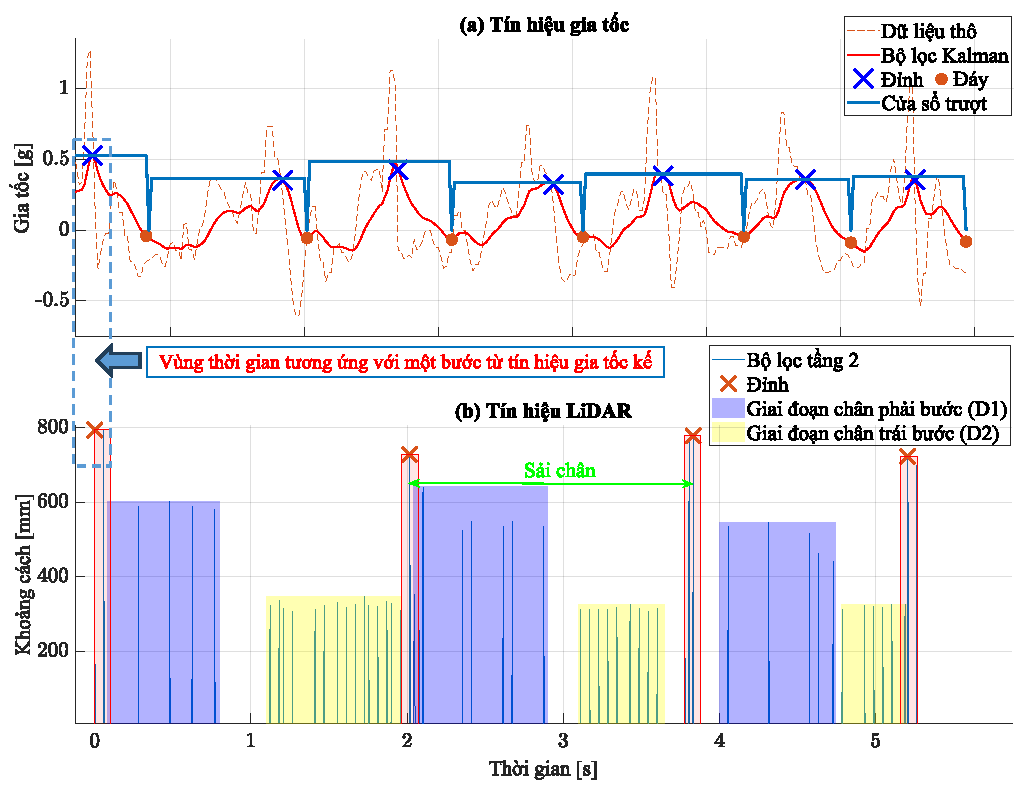
\includegraphics[width=1\linewidth]{Figure/acc_lidar.pdf}
    \caption{Bộ đếm bước được tích hợp để xác định thời điểm bước và hợp nhất với LiDAR nhằm loại bỏ các bước chân giả}
    \label{acc_lidar}
\end{figure}

Bộ đếm bước đóng vai trò quan trọng trong INS, đặc biệt là trong việc phát hiện chính xác số bước chân, từ đó cung cấp thông tin thiết yếu về quãng đường đã di chuyển và hỗ trợ định vị trong nhà cho nhân viên cứu hộ. Các thuật toán đếm bước chân được sử dụng phổ biến trong các môi trường hạn chế, cho phép xác định vị trí đối tượng dựa trên các phép đo từ gia tốc kế và con quay hồi chuyển. Một nghiên cứu trước đây đã đề xuất việc sử dụng cảm biến gia tốc ADXL345 và thuật toán phát hiện bước chân dựa trên kỹ thuật cửa sổ động để trích xuất các đoạn tín hiệu bước chân, kết hợp với bộ lọc Kalman để giảm nhiễu và bộ phân loại cây quyết định để nhận dạng bước chân~\cite{dao2023developing}. Kết quả thực nghiệm cho thấy phương pháp này đạt được các chỉ số đánh giá cao, với sai số tuyệt đối trung bình (Mean Absolute Error - MAE) là 0,333, sai số bình phương trung bình gốc chuẩn hóa (Normalized Root Mean Squared Error - NRMSE) là 0,008 và hệ số xác định R-squared đạt 0,999. Những phát hiện này khẳng định độ chính xác và độ tin cậy của phương pháp đếm bước đã đề xuất trên cả dữ liệu công khai và dữ liệu thực tế.

Trong nghiên cứu này, để khắc phục những hạn chế cố hữu khi chỉ sử dụng IMU hoặc LiDAR riêng lẻ, phương pháp hợp nhất dữ liệu từ cả hai cảm biến đã được đề xuất. Cụ thể, khi chỉ dựa vào IMU để định vị, hệ thống dễ gặp phải sai số tích lũy do trôi dạt cảm biến và sai số từ mô hình chuyển đổi dữ liệu quán tính thành quãng đường di chuyển. Mặt khác, LiDAR mặc dù có khả năng đo đạc chính xác tới từng milimet nhưng vẫn dễ bị nhiễu bởi các vật thể ngoài ý muốn trong không gian quét, gây ra các phép đo sai lệch.

Do đó, nghiên cứu này phát triển một chiến lược hợp nhất dữ liệu từ bộ đếm bước IMU và LiDAR thông qua bộ lọc đa giai đoạn. Thuật toán đếm bước sử dụng gia tốc kế sẽ xác định thời điểm bước chân, qua đó tạo ra các tín hiệu khởi phát (trigger) cho thuật toán phát hiện đỉnh từ dữ liệu LiDAR. Bằng cách này, các bước chân giả do nhiễu hoặc các dao động bất thường từ LiDAR có thể được loại bỏ, đồng thời các bước chân hợp lệ sẽ được nhận diện chính xác hơn. Hình~\ref{acc_lidar} minh họa quy trình hợp nhất dữ liệu từ IMU và LiDAR để xác định thời điểm bước chân và loại bỏ các bước chân giả, qua đó nâng cao độ tin cậy trong việc ước lượng khoảng cách bước chân và tổng quãng đường di chuyển.